\documentclass[11pt,openany]{article}
\usepackage{mathtools, commath}
% Packages for formatting
\usepackage[margin=1in]{geometry}
\usepackage{fancyhdr}
\usepackage{enumerate}
\usepackage{graphicx}
\usepackage{kotex}
\usepackage{arydshln} % Include this package
\usepackage{bbding}
\usepackage{amsmath}
\usepackage{amsthm}
\usepackage[dvipsnames,table]{xcolor}
\usepackage{amssymb, amsfonts}
\usepackage{wasysym}
\usepackage{footnote}
\usepackage{tablefootnote}
\usepackage{arydshln} % Include this package
% Fonts
\usepackage[T1]{fontenc}
\usepackage[utf8]{inputenc}
\usepackage{newpxtext,newpxmath}
\usepackage{sectsty}

\usepackage{array}  % Load the array package

% Define a new column type 'L' for left alignment with a specified width
\newcolumntype{L}[1]{>{\raggedright\arraybackslash}p{#1}}

% Define colors
\definecolor{TealBlue1}{HTML}{0077c2}
\definecolor{TealBlue2}{HTML}{00a5e6}
\definecolor{TealBlue3}{HTML}{b3e0ff}
\definecolor{TealBlue4}{HTML}{00293c}
\definecolor{TealBlue5}{HTML}{e6f7ff}

\definecolor{thmcolor}{RGB}{231, 76, 60}
\definecolor{defcolor}{RGB}{52, 152, 219}
\definecolor{lemcolor}{RGB}{155, 89, 182}
\definecolor{corcolor}{RGB}{46, 204, 113}
\definecolor{procolor}{RGB}{241, 196, 15}

\usepackage{color,soul}
\usepackage{soul}
\newcommand{\mathcolorbox}[2]{\colorbox{#1}{$\displaystyle #2$}}
\usepackage{cancel}
\newcommand\crossout[3][black]{\renewcommand\CancelColor{\color{#1}}\cancelto{#2}{#3}}
\newcommand\ncrossout[2][black]{\renewcommand\CancelColor{\color{#1}}\cancel{#2}}

\usepackage{hyperref}
\usepackage{booktabs}

% Chapter formatting
\definecolor{titleTealBlue}{RGB}{0,53,128}
\usepackage{titlesec}
\titleformat{\section}
{\normalfont\sffamily\LARGE\bfseries\color{titleTealBlue!100!gray}}{\thesection}{1em}{}
\titleformat{\subsection}
{\normalfont\sffamily\Large\bfseries\color{titleTealBlue!75!gray}}{\thesubsection}{1em}{}
\titleformat{\subsubsection}
{\normalfont\sffamily\large\bfseries\color{titleTealBlue!50!gray}}{\thesubsubsection}{1em}{}

%Tcolorbox
\usepackage[most]{tcolorbox}
\usepackage{multirow}
\usepackage{multicol}

\usepackage{caption}

\usepackage[linesnumbered,ruled]{algorithm2e}
\usepackage{algpseudocode}
\usepackage{setspace}
\SetKwComment{Comment}{/* }{ */}
\SetKwProg{Fn}{Function}{:}{end}
\SetKw{End}{end}
\SetKw{DownTo}{downto}

% Define a new environment for algorithms without line numbers
\newenvironment{algorithm2}[1][]{
	% Save the current state of the algorithm counter
	\newcounter{tempCounter}
	\setcounter{tempCounter}{\value{algocf}}
	% redefine the algorithm numbering (remove prefix)
	\renewcommand{\thealgocf}{}
	\begin{algorithm}
	}{
	\end{algorithm}
	% Restore the algorithm counter state
	\setcounter{algocf}{\value{tempCounter}}
}

\usepackage{adjustbox}
% Header and footer formatting
\pagestyle{fancy}
\fancyhead{}
\fancyhf{}
\lhead{\textcolor{TealBlue2}{\large\textbf{Crypto \& Security Engineering Lab}}}
\rhead{\textcolor{TealBlue2}{\large\textbf{[Research] Jasmin Language}}}%\rule{3cm}{0.4pt}}
% Define footer
%\newcommand{\footer}[1]{
%\begin{flushright}
%	\vspace{2em}
%	\includegraphics[width=2.5cm]{school_logo.jpg} \\
%	\vspace{1em}
%	\textcolor{TealBlue2}{\small\textbf{#1}}
%\end{flushright}
%}
%\rfoot{\large Department of Information Security, Cryptogrphy and Mathematics, Kookmin Uni.\includegraphics[height=1.5cm]{school_logo.jpg}}
\fancyfoot{}
\fancyfoot[C]{-\thepage-}

\usepackage{tabularx}
\usepackage{longtable}
\usepackage{array}
\usepackage{tcolorbox}
\tcbset{colback=white, arc=5pt}

\definecolor{defcolor}{RGB}{52, 152, 219}
\definecolor{procolor}{RGB}{241, 196, 15}
\definecolor{thmcolor}{RGB}{231, 76, 60}
\definecolor{lemcolor}{RGB}{155, 89, 182}
\definecolor{corcolor}{RGB}{46, 204, 113}
\definecolor{execolor}{RGB}{90, 128, 127}

% Define a new command for the custom tcolorbox
\newcommand{\defbox}[2][]{%
	\begin{tcolorbox}[colframe=defcolor, title={\color{white}\bfseries #1}]
		#2
	\end{tcolorbox}
}

\newcommand{\lembox}[2][]{%
	\begin{tcolorbox}[colframe=lemcolor, title={\color{white}\bfseries #1}]
		#2
	\end{tcolorbox}
}

\newcommand{\probox}[2][]{%
	\begin{tcolorbox}[colframe=procolor, title={\color{white}\bfseries #1}]
		#2
	\end{tcolorbox}
}

\newcommand{\thmbox}[2][]{%
	\begin{tcolorbox}[colframe=thmcolor, title={\color{white}\bfseries #1}]
		#2
	\end{tcolorbox}
}

\newcommand{\corbox}[2][]{%
	\begin{tcolorbox}[colframe=corcolor, title={\color{white}\bfseries #1}]
		#2
	\end{tcolorbox}
}
\usepackage{listings}
\definecolor{keyword}{HTML}{8e4e9e}
\definecolor{myblue}{HTML}{3471d8}
\definecolor{type}{HTML}{4EC9B0}
\definecolor{golden}{HTML}{d19a66}

% Change "Listing" to another name, e.g., "Code"
\renewcommand{\lstlistingname}{Code}
\lstdefinestyle{normal}{
%	frame=single, % Border
%	basicstyle=\tt\small, % Code font style
%	breaklines=true, % Break long lines into multiple lines automatically
%	aboveskip=1.5\baselineskip, % Vertical whitespace before the listing
	tabsize=3, % How many space to a tab
	upquote=true,
	mathescape=false,
	columns=fullflexible,
	keepspaces=true,
	captionpos=b,
	frame=tb,
	rangebeginprefix={(**\ begin\ },
	rangeendprefix={(**\ end\ },
	rangesuffix={\ *)},
	includerangemarker=false,
	basicstyle=\small\ttfamily,
	identifierstyle={},
	keywordstyle=[1]{\bfseries\color{violet}},
	keywordstyle=[2]{\bfseries\color{olive}},
	keywordstyle=[3]{\bfseries\color{blue}},
	keywordstyle=[4]{\bfseries\color{blue}},
	keywordstyle=[5]{\bfseries\color{red}},
	keywordstyle=[6]{\bfseries\color{violet}},
}
\lstdefinestyle{c}{
	language=C,
	basicstyle=\ttfamily\small,        % Basic font style
	keywordstyle=\color{keyword}\bfseries,       % Keywords in bold blue
	keywordstyle=[2]\color{myblue}\bfseries,
	keywordstyle=[3]\color{magenta}\bfseries,
	keywordstyle=[4]\color{purple}\bfseries,
	stringstyle=\color{red!70},               % Strings in reddish color
	commentstyle=\color{green!50!black}\itshape, % Comments in italic green-black
	numberstyle=\tiny\color{gray},            % Line numbers in tiny gray font
	numbers=left,                             % Line numbers on the left
	stepnumber=1,                             % Number every line
	numbersep=8pt,                            % Space between line numbers and code
%	backgroundcolor=\color{gray!10},          % Light gray background
	frame=single,                             % Single-line frame around the code
	rulecolor=\color{gray},                   % Frame color
	tabsize=4,                                % Tab space width
	showstringspaces=false,                   % Don't show spaces in strings
	breaklines=true,                          % Line breaking enabled
	breakatwhitespace=true,                   % Break lines at whitespace
	captionpos=b,                             % Caption below the code
	escapeinside={\%*}{*)},                   % Allow LaTeX within code
	morekeywords={printf, scanf, main, size_t, uint8_t, uint16_t, uint32_t, uint64_t},
	morekeywords=[2]{randomSeed, hashArray,
	expandChallenge, expandATF_vec_copy, expandColumns, expandSeeds,
	invertingOnATF, actingOnATFS, columnsMatrix, columnsDecomposition,
	multiplicationModuloP, addmul_P32_into_64, reductionModuloP,
	reductionStrict, inversionModuloP},
	morekeywords=[3]{crypto_sign_keypair, crypto_sign},
	morekeywords=[4]{lu}
}
% Command to Include Rust Code
\newcommand{\ccode}[2][]{%
	\lstinputlisting[style=c,#1]{#2}
}

% Inline Code Highlighting
\newcommand{\cinline}[1]{%
	\lstinline[style=c]|#1|%
}
\lstdefinestyle{asm}{
	%	language=[x86masm]Assembler,
	language=C,
	basicstyle=\ttfamily\small,
	keywordstyle=\color{blue},
	commentstyle=\color{gray!50},
	stringstyle=\color{orange},
	morekeywords={.data, .align, .asciz, .text, .global, .type, .size, .extern, stp, mov, adr, ldr, add, bl, ret, ldp, and,
	movk, lsr, mul, sub, uxtw, cmp, blt, str, cbnz},
	numbers=none,
	frame=single,                             % Single-line frame around the code
	rulecolor=\color{gray},                   % Frame color
}

%\lstdefinestyle{jasmin}{
%	language=[x86masm]Assembler, % Closest to Jasmin syntax
%	basicstyle=\ttfamily\small, % Monospace font for code
%	keywordstyle=\color{blue}\bfseries, % Keywords in blue and bold
%	stringstyle=\color{orange}, % Strings in orange
%	commentstyle=\color{green!60!black}\itshape, % Comments in green
%	numbers=left, % Line numbers on the left
%	numberstyle=\tiny\color{gray}, % Line number style
%	stepnumber=1, % Show every line number
%	numbersep=5pt, % Space between numbers and code
%	frame=single, % Single frame around code
%	tabsize=4, % Tab width
%	showstringspaces=false, % Don't underline spaces in strings
%	breaklines=true, % Wrap long lines
%	captionpos=b, % Caption at the bottom
%	morekeywords={mov, add, sub, mul, xor, and, or, shl, shr, call, ret, lea}, % Add Jasmin-specific keywords
%	escapeinside={(*@}{@*)} % For embedding LaTeX inside code
%}



%
%% --------------------------------------------------------------------
%\newcommand{\dslash}{\mathbin{\mathsf{/\mkern-4mu/}}}
%\newcommand{\dslasheq}{\mathbin{\mathsf{/\mkern-4mu/\mkern-8mu=}}}
%\newcommand{\slasheq}{\mathbin{\mathsf{/\mkern-6mu=}}}

% --------------------------------------------------------------------
\definecolor{OliveGreen}{rgb}{0.33, 0.5, 0.18}
\definecolor{Blue}{rgb}{0.06, 0.2, 0.65}
\definecolor{grey}{rgb}{0.43, 0.5, 0.5}
\lstdefinestyle{jasmin}{
	mathescape=true,
	columns=fullflexible,
	keepspaces=true,
	captionpos=b,
	frame=tb,
%	xleftmargin=.1\textwidth,
%	xrightmargin=.1\textwidth,
	rangebeginprefix={(**\ begin\ },
	rangeendprefix={(**\ end\ },
	rangesuffix={\ *)},
	includerangemarker=false,
	basicstyle=\small\sffamily,
	identifierstyle={},
	keywordstyle=[1]{\color{OliveGreen}},
	keywordstyle=[2]{\color{keyword}\bfseries},
	keywordstyle=[3]{\color{Blue}},
	keywordstyle=[4]{\bfseries\color{OliveGreen}},
	keywordstyle=[5]{\color{Red}},
	keywordstyle=[6]{\color{golden}},
	keywordstyle=[7]{\bfseries\color{magenta}},
%	morekeywords=[7]{xor, aes, enc, dec},
	morekeywords=[2]{fn,for,to,downto,if,else,do,while,return,param},
	morekeywords=[3]{u256,u128,u64,u32,u16,u8,bool,int},
	morekeywords=[1]{reg,stack,inline,export},
	comment=[l][\color{grey}]{//},
	morecomment=[s][\color{grey}]{/*}{*/},
	alsoletter ={_},
	literate=
	{-}{-}{1}%
	{->}{$\rightarrow$}{1}%
	{4u64}{4u64}{1}%
	{>>}{$\gg$}{1}%
	{<<}{$\ll$}{1}%,
}[keywords,comments]
\newcommand{\jasmincode}[2][]{%
	\lstinputlisting[style=jasmin,#1]{#2}
}
\newcommand{\jasmininline}[1]{%
	\lstinline[style=jasmin]|#1|%
}

\newcommand{\dslash}{\mathbin{\mathsf{/\mkern-4mu/}}}
\newcommand{\dslasheq}{\mathbin{\mathsf{/\mkern-4mu/\mkern-8mu=}}}
\newcommand{\slasheq}{\mathbin{\mathsf{/\mkern-6mu=}}}
\newcommand{\drarrow}{\raisebox{.07em}{$\mathbin{\scriptstyle\mathsf{-\mkern-3mu>}}$}}
\newcommand{\dlarrow}{\raisebox{.07em}{$\mathbin{\scriptstyle\mathsf{<\mkern-3mu-}}$}}
\newcommand{\drrarrow}{\raisebox{.07em}{$\mathbin{\scriptstyle\mathsf{-\mkern-3mu>\mkern-3mu>}}$}}
\newcommand{\dllarrow}{\raisebox{.07em}{$\mathbin{\scriptstyle\mathsf{<\mkern-3mu<\mkern-3mu-}}$}}
\lstdefinestyle{easycrypt}{
	upquote=true,
%	escapechar=\#,
	mathescape=false,
	columns=fullflexible,
	keepspaces=true,
	captionpos=b,
	frame=tb,
%	xleftmargin=.1\textwidth,
%	xrightmargin=.1\textwidth,
	rangebeginprefix={(**\ begin\ },
	rangeendprefix={(**\ end\ },
	rangesuffix={\ *)},
	includerangemarker=false,
	basicstyle=\small\ttfamily,
	identifierstyle={},
	keywordstyle=[1]{\bfseries\color{violet}},
	keywordstyle=[2]{\bfseries\color{olive}},
	keywordstyle=[3]{\bfseries\color{blue}},
	keywordstyle=[4]{\bfseries\color{blue}},
	keywordstyle=[5]{\bfseries\color{red}},
	keywordstyle=[6]{\bfseries\color{violet}},
	morekeywords=[1]{arg},
	morecomment=[n][\itshape]{(*}{*)},
	morecomment=[n][\bfseries]{(**}{*)},
	morekeywords=[1]{forall,exists,fun,glob,let,in,var,proc,if,then,else,elif,while,assert,return,res,equiv,hoare,phoare,islossless,async},
	morekeywords=[2]{axiom,axiomatized,lemma,realize,proof,qed,abort,goal,end,import,export,include,local,declare,hint,nosmt,module,of,const,op,pred,inductive,notation,abbrev,require,theory,abstract,section,type,class,instance,print,search,as,Pr,clone,with,rename,prover,timeout,why3,dump,remove,Top,Self},
	morekeywords=[3]{beta,iota,zeta,eta,logic,delta,simplify,congr,change,split,left,right,case,pose,cut,have,suff,elim,clear,wlog,apply,rewrite,rwnormal,subst,progress,trivial,auto,idtac,move,modpath,field,fieldeq,ring,ringeq,algebra,replace,transitivity,symmetry,seq,wp,sp,sim,skip,call,rcondt,rcondf,swap,cfold,rnd,pr_bounded,bypr,byphoare,byequiv,fel,conseq,exfalso,inline,alias,fission,fusion,unroll,splitwhile,kill,eager},
	morekeywords=[4]{try,first,last,do,strict,expect},
	morekeywords=[5]{exact,assumption,smt,by,reflexivity,done,solve},
	morekeywords=[6]{admit,admitted},
	literate=
	{tau}{$\tau$}1
	{sigma}{$\sigma$}1
	% note double "_" below
	% in actual EasyCrypt examples, do not use __
	% in specifications, these are rendered as subscripts
	{__1}{${}_{\!1}$}1
	{__2}{${}_{\!2}$}1
	{__3}{${}_{\!3}$}1
	{__n}{${}_{\!n}$}1
	{__p}{${}_{\!p}$}1
	{,,,}{$\mathrel{\ldots}$}1
	{...}{$\mathrel{\cdots}$}1
	{->}{$\drarrow$}1
	{<-}{$\dlarrow$}1
	{->>}{$\drrarrow$}2
	{<<-}{$\dllarrow$}2
}
\newcommand{\easycryptcode}[2][]{%
	\lstinputlisting[style=easycrypt,#1]{#2}
}
\newcommand{\easycryptinline}[1]{%
	\lstinline[style=easycrypt]|#1|%
}
\newcommand{\eccode}[2][]{%
	\lstinputlisting[style=easycrypt,#1]{#2}
}
\newcommand{\ecinline}[1]{%
	\lstinline[style=easycrypt]|#1|%
}

%\lstdefinestyle{easycrypt}{
%	language=ML, % EasyCrypt syntax is close to ML
%	basicstyle=\ttfamily\small, % Monospace font for code
%	keywordstyle=\color{purple}\bfseries, % Keywords in purple and bold
%	commentstyle=\color{green!60!black}, % Comments in green
%	stringstyle=\color{orange}, % Strings in orange
%	numbers=left, % Line numbers on the left
%	numberstyle=\tiny\color{gray}, % Line number style
%	stepnumber=1, % Show every line number
%	numbersep=5pt, % Space between numbers and code
%	frame=single, % Single frame around code
%	tabsize=4, % Tab width
%	showstringspaces=false, % Don't underline spaces in strings
%	breaklines=true, % Wrap long lines
%	captionpos=b, % Caption at the bottom
%	morekeywords={module, axiom, lemma, theorem, proof, qed, fun, let, in, forall, exists, if, then, else, return, assume, while, do, match, with}, % EasyCrypt-specific keywords
%	escapeinside={(*@}{@*)} % For embedding LaTeX inside code
%}
%\newcommand{\easycryptcode}[2][]{%
%	\lstinputlisting[style=easycrypt,#1]{#2}
%}
%\newcommand{\easycryptinline}[1]{%
%	\lstinline[style=easycrypt]|#1|%
%}
\usepackage{amsthm}

% Define custom theorem styles
\newtheoremstyle{dotless} % Name of the style
{3pt} % Space above
{3pt} % Space below
{\itshape} % Body font
{} % Indent amount
{\bfseries} % Theorem head font
{} % Punctuation after theorem head
{2.5mm} % Space after theorem head
{} % Theorem head spec

\newtheoremstyle{definitionstyle} % Name of the style
{3pt} % Space above
{3pt} % Space below
{} % Body font
{} % Indent amount
{\bfseries} % Theorem head font
{.} % Punctuation after theorem head
{2.5mm} % Space after theorem head
{} % Theorem head spec

% Applying custom styles
%\theoremstyle{dotless}
\newtheorem{theorem}{Theorem} % Theorem environment with section-wise numbering
\newtheorem*{theorem*}{Theorem} % Theorem environment with section-wise numbering
\newtheorem*{proposition*}{Proposition} % Theorem environment with section-wise numbering
\newtheorem*{corollary*}{Corollary} % Theorem environment with section-wise numbering
\newtheorem{proposition}[theorem]{Proposition} % Theorem environment with section-wise numbering
\newtheorem{lemma}[theorem]{Lemma} % Lemma shares the counter with theorem
\newtheorem{corollary}[theorem]{Corollary} % Corollary shares the counter with theorem

\theoremstyle{definitionstyle}
\newtheorem*{statement}{\textcolor{orange}{Statement}}
\newtheorem*{analysis}{\textcolor{magenta}{Analysis}}
\newtheorem*{pftactics}{\textcolor{teal}{Proof Tactics}}
\newtheorem*{observation}{\textcolor{Magenta}{Observation}}
\newtheorem{definition}{Definition} % Definition shares the counter with theorem
\newtheorem{example}{Example} % Example shares the counter with theorem
\newtheorem{exercise}{{Exercise}} % Example shares the counter with theorem
\newtheorem{remark}{Remark} % Remark shares the counter with theorem
\newtheorem*{note}{Note}

\newtheorem*{axiom*}{Axiom}
\newtheorem*{definition*}{Definition} % Definition shares the counter with theorem
\newtheorem*{example*}{Example} % Example shares the counter with theorem
\newtheorem*{exercise*}{\textcolor{violet}{Exercise}} % Example shares the counter with theorem
\newtheorem*{remark*}{Remark} % Remark shares the counter with theorem


\usepackage{tikz}
\usepackage{tikz-cd}
\usepackage{tikz-3dplot}
\def\Circlearrowleft{\ensuremath{%
		\rotatebox[origin=c]{180}{$\circlearrowleft$}}}
\def\Circlearrowright{\ensuremath{%
		\rotatebox[origin=c]{180}{$\circlearrowright$}}}
\def\CircleArrowleft{\ensuremath{%
		\reflectbox{\rotatebox[origin=c]{180}{$\circlearrowleft$}}}}
\def\CircleArrowright{\ensuremath{%
		\reflectbox{\rotatebox[origin=c]{180}{$\circlearrowright$}}}}
\usetikzlibrary{
	3d, % For 3D drawing
	angles,
	arrows,
	arrows.meta,
	backgrounds,
	bending,
	calc,
	decorations.pathmorphing,
	decorations.pathreplacing,
	decorations.markings,
	fit,
	matrix,
	patterns,
	patterns.meta,
	positioning,
	quotes,
	shadows,
	shapes,
	shapes.geometric,
	trees
}

\usepackage{pgfplots}
\pgfplotsset{compat=newest} % Adjust to your version of pgfplots
\usepgfplotslibrary{statistics}
% Commands for Research
\newcommand{\PRP}{\text{\normalfont PRP}}
\newcommand{\adversary}{\mathcal{A}}
\newcommand{\Adv}{\text{\normalfont Adv}}
\newcommand{\negl}{\text{\normalfont negl}}
\newcommand{\plaintext}{\mathcal{P}}
\newcommand{\messagespace}{\mathcal{M}}
\newcommand{\ciphertext}{\mathcal{C}}
\newcommand{\keyspace}{\mathcal{K}}
\newcommand{\encryption}{\mathcal{E}}
\newcommand{\decryption}{\mathcal{D}}
\newcommand{\nonce}{\mathcal{N}}
\newcommand{\keygen}{\mathsf{KeyGen}}
\newcommand{\enc}{\mathsf{Enc}}
\newcommand{\dec}{\mathsf{Dec}}
\newcommand{\uniform}{\xleftarrow{\$}}

% Commands for EasyCrypt
% Tools
\definecolor{eccolor}{HTML}{0f55bc}
\newcommand{\EasyCrypt}{{\bfseries\color{eccolor}\textsf{EasyCrypt}}\xspace}
\newcommand{\EC}{{\bfseries\color{eccolor}\textsf{EC}}\xspace}
\newcommand{\OCaml}{{\bfseries\textsf{OCaml}}\xspace}
\newcommand{\Emacs}{{\bfseries\textsf{Emacs}}\xspace}
\newcommand{\ZThree}{{\bfseries\textsf{Z3}}\xspace}
\newcommand{\CVCFour}{{\bfseries\textsf{CVC4}}\xspace}
\newcommand{\AltErgo}{{\bfseries\textsf{Alt-ergo}}\xspace}
\newcommand{\ProofGeneral}{{\bfseries\textsf{Proof General}}\xspace}
\newcommand{\CertiCrypt}{\textsf{CertiCrypt}\xspace}
\newcommand{\CertiPriv}{\textsf{CertiPriv}\xspace}
\newcommand{\SsReflect}{\textsf{SsReflect}\xspace}
\newcommand{\Coq}{{\bfseries\textsf{Coq}}\xspace}
\newcommand{\WhyThree}{{\bfseries\textsf{Why3}}\xspace}
\newcommand{\SMT}{{\bfseries\textsf{SMT}}\xspace}
% Languages and Logics
\newcommand{\pWHILE}{\textsf{p}\textsc{While}\xspace}
\newcommand{\pRHL}{\textsf{pRHL}\xspace}
% Version numbers
\newcommand{\ECversion}{1.0\xspace}
%% Misc
\newcommand{\DONE}{}% {{\color{red}DONE}}
\newcommand{\Example}{\paragraph*{Example}}
\newcommand{\Syntax}{\paragraph*{Syntax}}
\newcommand{\Description}{\paragraph*{Description}}
\newcommand{\INDRoR}{\textsf{IND-RoR}\xspace}
\newcommand{\INDCPA}{\textsf{IND-CPA}\xspace}
\newcommand{\INDCCAone}{\textsf{IND-CCA1}\xspace}
\newcommand{\INDCCA}{\textsf{IND-CCA}\xspace}
\newcommand{\EFCMA}{\textsf{EF-CMA}\xspace}
\newcommand{\LCDH}{\ensuremath{\mathsf{LCDH}}\xspace}
\newcommand{\CDH}{\textsf{CDH}\xspace}
\newcommand{\DDH}{\textsf{DDH}\xspace}
\newcommand{\ElGamal}{\textsf{ElGamal}\xspace}
\newcommand{\HElGamal}{\textsf{HElGamal}\xspace}
\newcommand{\RSA}{\textsf{RSA}\xspace}
\newcommand{\OAEP}{\textsf{OAEP}\xspace}
\newcommand{\FDH}{\textsf{FDH}\xspace}
\newcommand{\HMAC}{\textsf{HMAC}\xspace}
\newcommand{\CS}{\textsf{CS}\xspace}
\newcommand{\Skein}{\textsf{Skein}\xspace}
\newcommand{\TCR}{\textsf{TCR}\xspace}

\newcommand{\KG}{\mathcal{KG}}
\newcommand{\Enc}{\mathcal{E}}
\newcommand{\Dec}{\mathcal{D}}

%%% Complexity and termination
%\newcommand{\lossless}{\mathsf{lossless}}

%%% Sets
%\newcommand{\zeroone}{[0,1]}
%\newcommand{\bit}{\{0,1\}}
%\newcommand{\bitstring}[1]{\ensuremath{\bit^{#1}}}
%\newcommand{\bool}{\mathbb{B}}
%\newcommand{\nat}{\mathbb{N}}
%\newcommand{\real}{\mathbb{R}}
%\newcommand{\option}[1]{#1_\bot}
%
%%% Mathematics
%\newcommand{\conv}[1][]{\mathrel{\leftrightarrow^*_{#1}}}
%\renewcommand{\Pr}[2]{\mathrm{Pr}\left[#1 : #2\right]}
%\newcommand{\Prm}[3]{\mathrm{Pr}\left[#1,#3 : #2\right]}
%\newcommand{\labs}{\left\lvert}
%\newcommand{\rabs}{\right\rvert}
%\newcommand{\charfun}{\mathds{1}}

%% Distribution monad
%\newcommand{\supp}{\mathsf{support}}
%\newcommand{\range}[2]{\mathsf{range}~{#1}~{#2}}

%% Semantics 

% \newcommand{\sem}[1]{\llbracket #1 \rrbracket}
%\newcommand{\subst}[2]{\left[{}^{#2}/{}_{#1}\right]}
%\newcommand{\fv}{\mathsf{fv}}
%\newcommand{\modifies}{\mathsf{mod}}
%\newcommand{\glob}{\mathsf{glob}}
%\newcommand{\Env}{\mathcal{E}}

%%% Well-formed adversaries
%%% Program Judgements 
\newcommand{\Hoare}[3]{\left[{#1}:{#2}\Longrightarrow{#3}\right]}
%\newcommand{\Equiv}[4]{\left[{#1}\sim{#2}:{#3}\Longrightarrow{#4}\right]}
%\newcommand{\bdHoareS}[5]{{\Hoare{#1}{#2}{#3}}\,{#4}\,{#5}}
%\newcommand{\HoareLe}[4]{\bdHoareS{#1}{#2}{#3}{\leq}{#4}}
%\newcommand{\HoareEq}[4]{\bdHoareS{#1}{#2}{#3}{=}{#4}}
%\newcommand{\HoareGe}[4]{\bdHoareS{#1}{#2}{#3}{\geq}{#4}}
%
%
%% \newcommand{\Equiv}[4]{\models {#1} \sim {#2} : {#3} \Longrightarrow {#4}}
%% \newcommand{\AEquiv}[6]{\models {#2} \sim_{#5,#6} {#3} : {#1} \Longrightarrow {#4}}
%% \newcommand{\JAEquiv}[6]{{#2} \sim_{#5,#6} {#3} : {#1} \Longrightarrow {#4}}
%% \newcommand{\EquivMem}[2]{\models {#1} \equiv {#2}}
%% \newcommand{\EqObs}[4]{\models {#1} \simeq^{#3}_{#4} {#2}}
%% \newcommand{\AEqObs}[5]{\models {#1} \simeq^{#3}_{{#4}} {#2} \preceq {#5}} 
%% \newcommand{\ACEqObs}[7]
%%         {\AEqObs{\left[ #1 \right]_{#6}}{\left[ #2 \right]_{#7}}{#3}{#4}{#5}}
%% \newcommand{\Triple}[3]{\sem{#2} {#3} \preceq {#1}}
%% \newcommand{\DTriple}[3]{\sem{#2} {#3} \succeq {#1}}
%% \newcommand{\dequiv}[3]{{#1} \simeq_{#3} {#2}}
%% \newcommand{\fequiv}[3]{{#1} =_{#3} {#2}}
%% \newcommand{\Pre}{\Psi}
%% \newcommand{\Post}{\Phi}
%% \newcommand{\Inv}{\Phi}
%\newcommand{\side}[1]{\langle #1 \rangle}
%\newcommand{\sidel}{\side{1}}
%\newcommand{\sider}{\side{2}}
%% \newcommand{\eqobsin}{\mathsf{eqobs\_in}}
%% \newcommand{\eqobsout}{\mathsf{eqobs\_out}}
%\newcommand{\pre}{\Psi}
%\newcommand{\post}{\Phi}
%\newcommand{\bound}{\delta}
%\newcommand{\ECinsupp}[2]{\mathec{Distr.in_supp}\,{#1}\,{#2}}
%\newcommand{\insupp}[2]{{#1}\in\mathec{supp}\,{#2}}
%%% Variables
%
%% \newcommand{\LH}{\gl{L}_H}
%% \newcommand{\LD}{\gl{L}_\Dec}
%% \newcommand{\cdef}{\gl{\gamma_\mathsf{def}}}
%\newcommand{\var}[1]{\ensuremath{\mathit{#1}} \xspace}

%% Constants and operators
% TODO: Update!
%\newcommand{\true}{\mathsf{true}}
%\newcommand{\false}{\mathsf{false}}
%\newcommand{\nil}{\mathsf{nil}}
%\newcommand{\hd}{\mathsf{hd}}
%\newcommand{\tl}{\mathsf{tl}}
%\newcommand{\app}{\mathbin{+\mkern-7mu+}}
%\newcommand{\concat}{\parallel}
%\newcommand{\xor}{\oplus}
%\newcommand{\msb}[2]{[#1]^{#2}}
%\newcommand{\lsb}[2]{[#1]_{#2}}
%\newcommand{\dom}{\mathsf{dom}}
%\newcommand{\ran}{\mathsf{ran}}
%\newcommand{\fst}{\mathsf{fst}}
%\newcommand{\snd}{\mathsf{snd}}
%\newcommand{\some}[1]{#1}
%\newcommand{\none}{\bot}
%
%\newcommand{\Int}{\mathsf{Int}}
%\newcommand{\tint}{\mathsf{int}}
%
%\newcommand{\tbool}{\mathsf{bool}}


%
\newcommand{\plain}{\mathcal{P}}
\newcommand{\key}{\mathcal{K}}
\newcommand{\authen}{\mathcal{A}}
\newcommand{\signature}{\mathcal{S}}
\newcommand{\verification}{\mathcal{V}}
\newcommand{\sig}{\textbf{sig}}
\newcommand{\ver}{\textbf{ver}}

\newcommand{\ie}{\textnormal{i.e.}}
\newcommand{\rsa}{\mathsf{RSA}}
\newcommand{\rsacrt}{\mathsf{RSA}\textendash\mathsf{CRT}}
\newcommand{\inv}[1]{#1^{-1}}

%New Command
%\newcommand{\set}[1]{\left\{#1\right\}}
\newcommand{\N}{\mathbb{N}}
\newcommand{\Z}{\mathbb{Z}}
\newcommand{\Q}{\mathbb{Q}}
\newcommand{\R}{\mathbb{R}}
\newcommand{\cR}{\mathcal{R}}
\newcommand{\C}{\mathbb{C}}
\newcommand{\F}{\mathbb{F}}
\newcommand{\nbhd}{\mathcal{N}}
\newcommand{\Log}{\operatorname{Log}}
\newcommand{\Arg}{\operatorname{Arg}}
\newcommand{\pv}{\operatorname{P.V.}}

\newcommand{\of}[1]{\left( #1 \right)} 
%\newcommand{\abs}[1]{\left\lvert #1 \right\rvert}
%\newcommand{\norm}[1]{\left\| #1 \right\|}

\newcommand{\sol}{\textcolor{magenta}{\bf Sol}}

\DeclarePairedDelimiter\ceil{\lceil}{\rceil}
\DeclarePairedDelimiter\floor{\lfloor}{\rfloor}


\newcommand{\cyclic}[1]{\langle #1 \rangle}
\newcommand{\xmark}{\textcolor{red}{\XSolidBrush}}
\newcommand{\vmark}{\textcolor{green!75!black}{\CheckmarkBold}}

\newcommand{\gen}[1]{\langle #1 \rangle}
\newcommand{\Gen}[1]{\left\langle #1 \right\rangle}

\newcommand{\img}[1]{\text{Img}(#1)}
\newcommand{\Img}[1]{\text{Img}\left(#1\right)}
\newcommand{\preimg}[1]{\text{Img}^{-1}(#1)}
\newcommand{\Preimg}[1]{\text{Img}^{-1}\left(#1\right)}

\newcommand{\relation}{\mathrel{\mathcal{R}}}
\newcommand{\injection}{\rightarrowtail}
\newcommand{\surjection}{\twoheadrightarrow}
\newcommand{\id}{\textnormal{id}}

\newcommand{\eqclass}[1]{\left[#1\right]}

% Define custom colors for O and X
\newcommand{\yes}{\textcolor{blue}{\bf \fullmoon}}
\newcommand{\no}{\textcolor{red}{\bf \texttimes}}


\usepackage{background}  % For setting background images

\backgroundsetup{
	scale=1,  % Scale the image to fit the page
	color=black,  % Keep the image color as is
	opacity=.1,  % Fully opaque background
	angle=0,  % No rotation
	vshift=1cm,  % Adjust vertical alignment if needed
	contents={}
}
\newcommand{\setPageBackground}{
	\backgroundsetup{
		contents={
\includegraphics[scale=4]{images/school-logo}}}
}

\setstretch{1.25}
\begin{document}
\begin{titlepage}
\setPageBackground  % Enable background image for title page
\begin{center}
	{\Huge{\textbf{EasyCrypt Library in Jasmin}}\par}
	{\LARGE\textbf{\textbf{v 1.0}}\par}
	\vspace{0.5in}
	{\LARGE {\textbf{Ji, Yong-hyeon}\\ (\texttt{hacker3740@kookmin.ac.kr})}\par}
	\vfill
	{\Large\bf \textsf{Department of Information Security, Cryptology, and Mathematics}\par}
	{\Large\textsf{College of Science and Technology}\par}
	{\Large\textsf{Kookmin University}\par}
	\vspace{.75in}
	
\includegraphics[scale=.35]{images/logo.png}\par
	\vspace{.25in}
	{\Large\textsf{\today}\par}
\end{center}
\end{titlepage}
\newpage

\subsection*{File Structure}
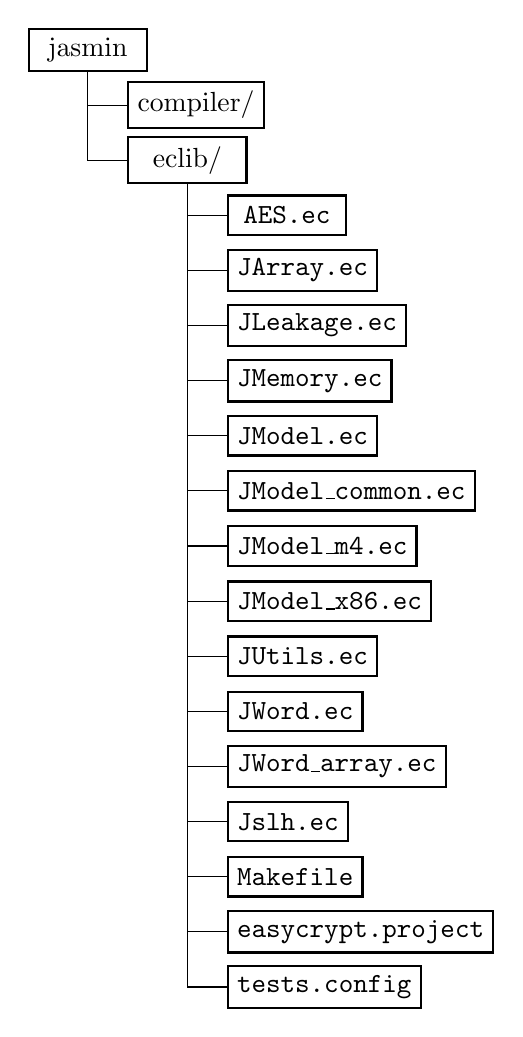
\begin{tikzpicture}[%
	grow via three points={one child at (0.5,-0.7) and
		two children at (0.5,-0.7) and (0.5,-1.4)},
	edge from parent path={(\tikzparentnode.south) |- (\tikzchildnode.west)}]
	\tikzstyle{every node}=[draw=black,thick,anchor=west, minimum width=1.5cm, minimum height=.5cm]
	\tikzstyle{selected}=[draw=red,fill=red!30]
	\tikzstyle{optional}=[dashed,fill=gray!50]
	\node {jasmin}
	child { node {compiler/} }	
	child { node {eclib/}
		child { node {\ttfamily AES.ec}}
		child { node {\ttfamily JArray.ec}}
		child { node {\ttfamily JLeakage.ec}}
		child { node {\ttfamily JMemory.ec}}
		child { node {\ttfamily JModel.ec}}
		child { node {\ttfamily JModel\_common.ec}}
		child { node {\ttfamily JModel\_m4.ec}}
		child { node {\ttfamily JModel\_x86.ec}}
		child { node {\ttfamily JUtils.ec}}
		child { node {\ttfamily JWord.ec}}
		child { node {\ttfamily JWord\_array.ec}}
		child { node {\ttfamily Jslh.ec}}
		child { node {\ttfamily Makefile}}
		child { node {\ttfamily easycrypt.project}}
		child { node {\ttfamily tests.config}}
	}
	child [missing] {}	
	child [missing] {}
	child [missing] {}	
	child [missing] {}	
	child [missing] {}	
	child [missing] {}	
	child [missing] {}	
	child [missing] {}	
	child [missing] {}	
	child [missing] {}	
	child [missing] {}	
	child [missing] {}	
	child [missing] {}	
	child [missing] {}	
	child [missing] {}	
%	child { node {src/} }
%	child { node {src/} }
%		child { node {aeslib/}
%			child { node {\texttt{aes.jazz}} }
%		}
%		child [missing] {}	
%		child { node {example/} 
%			child { node {\texttt{NbAESEnc.jazz}} }
%			child { node {\texttt{NbAESEnc\_mem.jazz}} }
%		}
%	}
%	child { node {compress.c}}
%	child { node {expand.c}}
%	child { node[selected] {field.c}}
%	child { node {matrix.c}}
%	child { node {sign.c}};
%	child { node [selected] {tex}
%		child { node {generic}}
%		child { node [optional] {latex}}
%		child { node {plain}}
%	};
;
\end{tikzpicture}

\vfill
\subsection*{Copyright}
%\large
\textcopyright~ 2024 Crypto and Security Engineering Lab
All rights reserved.

This document and its content are the intellectual property of ``Ji, Yong-hyeon''. No part of this document may be reproduced, distributed, or transmitted in any form or by any means, including photocopying, recording, or other electronic or mechanical methods, without the prior written permission of the author, except in the case of brief quotations embodied in critical reviews and certain other noncommercial uses permitted by copyright law. For permission requests, write to the author at the e-mail.

\vfill
\subsection*{Changelog}
\large
\begin{tabular}{@{} L{0.05\textwidth} L{0.2\textwidth} L{0.7\textwidth} @{}} % Column widths specified here, change as needed for your content
	\toprule
	v1.0 & 2025-01-03 & Initial release: \\%Implementation and benchmarks.\\
	%		v1.1 & 20XX-02-27 & Pellentesque iaculis odio vel nisl ullamcorper, nec faucibus ipsum molestie.\\
	%		v1.2 & 20XX-03-15 & Sed dictum nisl non aliquet porttitor.\\
	\bottomrule
\end{tabular}

\newpage

\pagenumbering{arabic}

\tableofcontents

\newpage
\section{AES}
\easycryptcode[linerange={1-1}]{listings/AES.ec}

\subsection{Operations on bytes and word}
\easycryptcode[linerange={5-8}]{listings/AES.ec}
\begin{itemize}
	\item $\texttt{Sbox}:\F_{2^8}\to\F_{2^8}$
	\item $\texttt{InvSbox}:\F_{2^8}\to\F_{2^8}$
	\item $\texttt{InvSbox}(\texttt{Sbox}(w))=w$, where $w\in\F_{2^8}$.
\end{itemize}
\easycryptcode[linerange={12-22}]{listings/AES.ec}
\begin{itemize}
	\item Let $w=[w_0,w_1,w_2,w_3]$, where $w_i\in\F_{2^8}$. Then \begin{align*}
		\texttt{SubWord}(w)&=[\texttt{Sbox}(w_0),\texttt{Sbox}(w_1),\texttt{Sbox}(w_2),\texttt{Sbox}(w_3)]
	\end{align*}
\end{itemize}

\newpage
\section{JUtils}
%\subsection{JUtils}
\easycryptcode[linerange={1-3}]{listings/JUtils.ec}

\begin{table}[h!]
\begin{tabular}{l}
\url{https://github.com/EasyCrypt/easycrypt}\\
easycrypt/theories/core/AllCore.ec\\
easycrypt/theories/core/Bool.ec\\
easycrypt/theories/algebra/IntDiv.ec\\
easycrypt/theories/algebra/StdOrder.ec\\
easycrypt/theories/datatypes/List.ec\\
\end{tabular}
\end{table}

\subsubsection*{LEMMA:\quad \texttt{modz\_comp}}
% modz_cmp
\easycryptcode[linerange={6-7}]{listings/JUtils.ec}
\begin{statement}
	For two integers $m$ and $d>0$, the remainder of 
	$m$ divided by $d$ satisfies:\[
	0\leq m\bmod d< d.
	\]
\end{statement}
\ \\
\begin{analysis}
	This property follows directly from the division algorithm: \[
	m=q\cdot d+r,\quad 0\leq r<d
	\] where $q=\floor*{m/d}$ and $r=m\bmod q$.
\end{analysis}
\ \\
\begin{pftactics}
	SMT solver with the pre-proved property \texttt{edivzP} (in \texttt{IntDiv}).
\end{pftactics}

\newpage
\subsubsection*{LEMMA:\quad \texttt{divz\_cmp}}
% divz_cmp
\easycryptcode[linerange={9-12}]{listings/JUtils.ec}
\begin{statement}
	For integers $d,i,n$ where $d>0$ and $0\leq i< n\cdot d$, the integer division satisfies \[
	0\leq \frac{i}{d}< n.
	\]
\end{statement}
\ \\
\begin{analysis}
	TBA
\end{analysis}
\ \\
\begin{pftactics}
	TBA
\end{pftactics}

\subsubsection*{LEMMA:\quad \texttt{mulz\_cmp\_r}}
% mulz_cmp_r
\easycryptcode[linerange={14-18}]{listings/JUtils.ec}
\begin{statement}
	TBA
\end{statement}
\ \\
\begin{analysis}
	TBA
\end{analysis}
\ \\
\begin{pftactics}
	TBA
\end{pftactics}

\subsubsection*{LEMMA:\quad \texttt{cmpW}}
% cmpW
\easycryptcode[linerange={20-21}]{listings/JUtils.ec}
\begin{statement}
	TBA
\end{statement}
\ \\
\begin{analysis}
	TBA
\end{analysis}
\ \\
\begin{pftactics}
	TBA
\end{pftactics}

\subsubsection*{LEMMA:\quad \texttt{le\_modz}}
% le_modz
\easycryptcode[linerange={23-30}]{listings/JUtils.ec}
\begin{statement}
	TBA
\end{statement}
\ \\
\begin{analysis}
	TBA
\end{analysis}
\ \\
\begin{pftactics}
	TBA
\end{pftactics}

\newpage
\section{JArray}
\input{sections/JArray}

%\newpage
\vfill
\begin{thebibliography}{9}\large
%	\bibitem{Introduction_to_Modern_Cryptography}
%	Jonathan, Katz. \textit{Introduction to Modern Cryptography, Second Edition}., n.d.
%	\bibitem{Cryptography_Made_Simple}
%	Smart, Nigel P. \textit{Cryptography Made Simple. Information Security and Cryptography}. Cham: Springer International Publishing, 2016. https://doi.org/10.1007/978-3-319-21936-3.
\end{thebibliography}

\newpage
\appendix
\section{Prelude}
\subsection{Logic}
\subsubsection*{Principle of Functional Extensionality}
\easycryptcode[linerange={60-60}]{listings/easycrypt/theories/prelude/Logic.ec}
The axiom asserts: \[
f=g\iff f==g
\]
\begin{itemize}
	\item Left-hand side $(f=g)$:
	
	This refers to the equality of functions as mathematical objects. Two functions 
	$f$ and $g$ are equal if they are identical, meaning they are the same function in every aspect.
	\item Right-hand side $(f==g)$:
	
	This refers to pointwise equality: 
	$f(x)=g(x)$ for all $x\in'a$
	\item Interpretation:
	
	The axiom establishes that two functions are equal as mathematical objects if and only if they produce the same output for every input. This is the essence of functional extensionality.
\end{itemize}

\begin{table}[h!]
\begin{tabularx}{\textwidth}{>{\raggedleft\arraybackslash}p{.15\textwidth}|p{.75\textwidth}}
\toprule[1.2pt]
Set Theory & In classical set theory (ZFC), functional extensionality is implicitly satisfied because functions are defined as sets of ordered pairs: \[
f=\set{(x,f(x)):x\in\text{dom}(f)}.
\] Thus, two functions are equal if and only if their values agree for every input. \\ \hline
Category Theory & In category theory, functional extensionality corresponds to the notion that morphisms (arrows) between objects are determined by their action on elements. \\ \hline
Constructive Mathematics & In constructive frameworks (e.g., type theory), functional extensionality may not hold by default, as functions can be defined by their computational behavior rather than just their input-output relations.\par
In such settings, extensionality is often treated as an additional axiom. \\
\bottomrule[1.2pt]
\end{tabularx}
\end{table}

\newpage
\subsubsection*{Constructive Choice Function}
\easycryptcode[linerange={645-658}]{listings/easycrypt/theories/prelude/Logic.ec}
\paragraph{Definition of \texttt{choiceb}} For a predicate $P:\texttt{'a}\to\set{\texttt{true},\texttt{false}}$ and a default element $x_0\in\texttt{'a}$, it selects an element $x\in\texttt{'a}$ such that $P(x)=\texttt{true}$, if such an $x$ exists. Otherwise, it defaults to $x_0$. That is, \[
\texttt{choiceb}(P,x_0)=
\begin{cases}
	x&:\exists x\in\texttt{'a}:P(x)=\texttt{true}\\
	x_0&:\forall x\in\texttt{'a}:P(x)=\texttt{false}\\
\end{cases}
\]
\paragraph{Axioms for \texttt{choiceP}} If there exists an element 
$x$ such that $P(x)=\texttt{true}$, then $\texttt{choiceb}(P,x_0)$
satisfies $P$, \ie, $P(\texttt{choiceb}(P,x_0))=\texttt{true}$.\par
This axiom asserts that the choice function correctly selects an element from the subset defined by $P$, whenever such an element exists. It embodies the constructive aspect of the function.
\paragraph{\texttt{choiceb\_dfl}} If $P(x)=\texttt{false}$ for all $x\in\texttt{'a}$, then 
$\texttt{choiceb}(P,x_0)$ returns the default value $x_0$.\par
This axiom ensures that the function $\texttt{choiceb}$ respects its fallback behavior when the subset defined by $P$ is empty.
\paragraph{Equality of Choices} If two predicates $P$ and $Q$ are logically equivalent (i.e., $P(x)\Leftrightarrow Q(x)$ for all $x\in\texttt{'a}$), then $\texttt{choiceb}(P,x_0)=\texttt{choiceb}(Q,x_0)$.\par
The proof relies on the extensionality of predicates: functions 
$P$ and $Q$ are equivalent if they have identical output for all inputs.
\paragraph{Axiom: Irrelevance of Default for Non-Empty Subsets} If $P$ is satisfied by some element $x$, the value of $\texttt{choiceb}(P,x_0)$ is independent of the default value $x_0$.\par
This axiom guarantees that when $\exists x\in\texttt{'a}:P(x)=\texttt{true}$, the choice function selects an element satisfying $P$, irrespective of the fallback $x_0$. This is because the fallback $x_0$ is only used when $P$ is unsatisfiable.\par
This property reflects the \textbf{stability} of the constructive choice under changes to the fallback parameter, provided the primary condition is satisfied.
\paragraph{Summary} These axioms and lemmas collectively define a constructive choice principle, a central concept in intuitionistic mathematics and proof systems. Unlike classical logic's unrestricted use of the axiom of choice, this constructive version ensures explicit constructability of the chosen element.
\paragraph{Application} This construct is useful in formal verification for:
\begin{itemize}
	\item Selecting elements satisfying a predicate (e.g., in search or optimization problems).
	\item Ensuring robust behavior under different edge cases (e.g., empty or singleton sets).
	\item Proving properties of algorithms that depend on choice.
\end{itemize}

\newpage
\section{Algebra}

\subsection{IntDiv}
\easycryptcode[linerange={17-37}]{listings/easycrypt/theories/algebra/IntDiv.ec}
\paragraph{Quotient (\easycryptinline{\%/})}
\paragraph{Remainder (\easycryptinline{\%\%})}
\paragraph{Divisibility (\easycryptinline{\%|})} $m\ \texttt{\%|} d\iff m\bmod d=0$.
%\paragraph{\texttt{euclidef}} The definition formalizes the Euclidean division, which states: For any integers $m\in\Z$ and $d\neq 0$, there exist unique integers 
%$q,r\in\Z$ such that: \[
%m=q\cdot d+r\quad\text{and}\quad 0\leq r<\abs{d}.
%\] Thus,
%\[
%\texttt{euclidef}(m,d,(q,r))\iff\begin{cases*}
%	m=q\cdot d+r\\
%	0\leq r<\abs{d}&if $d\neq 0$
%\end{cases*}
%\]
%\paragraph{\texttt{edivn}}
\paragraph{Applications} The modular arithmetic constructs are essential for reasoning about cryptographic algorithms (e.g., RSA, Diffie-Hellman).
Division and modulus operations are cornerstones for verifying number-theoretic properties.
\newpage
\easycryptcode[linerange={50-71}]{listings/easycrypt/theories/algebra/IntDiv.ec}
%\begin{tikzpicture}[node distance=2cm, on grid, auto]
%	
%	\node[state, initial] (start) {Start: Rewrite \texttt{edivz\_def}};
%	\node[state] (checkm) [below=of start] {Check \( 0 \leq m \)};
%	\node[state] (posm) [right=of checkm] {Case: \( 0 \leq m \)};
%	\node[state] (negm) [left=of checkm] {Case: \( 0 > m \)};
%	\node[state] (checkd) [below=of checkm] {Check \( d = 0 \)};
%	\node[state] (result) [below=of checkd] {Result: Prove lemma};
%	
%	\path[->]
%	(start) edge node {Rewrite} (checkm)
%	(checkm) edge node {If \( 0 \leq m \)} (posm)
%	(checkm) edge node {Else} (negm)
%	(posm) edge [bend right] node {Validate \( edivnP \)} (checkd)
%	(negm) edge [bend left] node {Validate \( edivnP \)} (checkd)
%	(checkd) edge node {If \( d = 0 \)} (result);
%	
%\end{tikzpicture}


%\input{appendices/mesure_cycle.tex}

\end{document}
